\begin{center}

  \begin{tabular}{rp{16cm}lp{20cm}}%{rl}

  % after \\: \hline or \cline{col1-col2} \cline{col3-col4} ...

  论文地址:& \href{https://openreview.net/pdf?id=rJeW1yHYwH}{https://openreview.net/pdf?id=rJeW1yHYwH} \\
  来源:& ICLR, 2020\\
  作者:& Da Xu, Chuanwei Ruan, et al. \\

  源码:& \href{https://github.com/StatsDLMathsRecomSys/Inductive-representation-learning-on-temporal-graphs}{TGAT} \\

%  slides:& \href{http://yunshengb.com/wp-content/uploads/2017/03/nips_2018_r2l_workshop_talk.pdf}{{\footnotesize Convolutional Set Matching for Graph Similarity}}\\

  关键词:& \textbf{self-attention mechanism, graph representation, temporal graph} \\

  写于:& \date{2021-03-01}

  \end{tabular}

\end{center}

该论文\cite{tgat_iclr20}也是为了解决动态图的表征问题。改论文在self-attention\cite{vaswani2017attention}机制的基础上,提出了temporal graph attention(TGAT) layer来汇集temporal-topological neighborhood features。

\paragraph{问题定义}
该论文讨论的也是连续时间下的动态图的表征问题,与\cite{rossi2020temporal}不同,该论文并没有将动态图用事件序列来表示,重点关注的时图中结点的temporal neighborhoods,如何利用temporal neighborhoods来计算结点在$t$时的表征。

\paragraph{TGAT思路}
在介绍TGAT之前,先来了解以下self-attention是啥。
\subparagraph{self-attention}
简单的来说自注意力机制就是输入一个序列的数据,以序列自身来计算序列中各个元素与其他元素(包括自身)之间的关系大小(注意力大小)。self-attention最开始用于自然语言处理中。在计算自注意力时需要将位置编码与序列中元素的表征相结合。
$$
Attn(Q, K, V) = softmax(\frac{\mathbf{Q}\mathbf{K}^\intercal}{\sqrt{d}}) \mathbf{V}
$$
上式中的$\mathbf{Q,K,V}$都是由同一个矩阵$\mathbf{X}$(表征矩阵)乘以不同的权重矩阵得到的。

\subparagraph{TGAT}
TGAT中将self-attention中的positional encoding替换为time encoding,再将time encoding与结点特征相结合构成Temporal Graph Attention Layer。time encoding的输入为时间戳,输出为一个向量。对于时间$t$,结点$i$的temporal neighborhoods包括在时间$t$之与$i$发生了交互(即存在过边)的结点,每个结点上一层的表征和时间表征拼接起来作为self-attention中的$\mathbf{X}$,即可计算得到当前节点与其temporal neighborhoods之间的注意力,邻居结点的上一层的表征加权求和后隐表示,该隐表示再与结点的特征向量拼接后输入到MLP中,最终的输出为节点在$t$时的TGAT层输出。TGAT layer如Fig.\ref{fig:tgat}所示。

\begin{figure}[h]
	\centering
	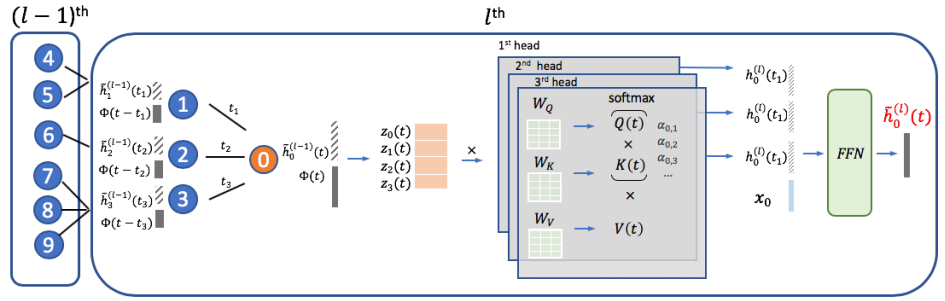
\includegraphics[width=.8\textwidth]{pics/TGAT.png}
	\caption{TGAT layer,采用了多头注意力机制,k=3}
	\label{fig:tgat}
\end{figure}

说实话,TAGT的大概意思看懂了,但是其中涉及time encoding转化为一个分布学习的问题、TGAT layer的具体实现过程不是很懂。






\paragraph{方法解决的问题/优势}

\begin{itemize}

	\item 引入了temporal的图注意力机制
	\item 将self-attention中的positional encoding替换为time encoding
	\item 引入了注意力机制能够增加模型的可解释性

\end{itemize}



\paragraph{方法的局限性/未来方向}

\begin{itemize}

	\item 对于$t$时的结点的表征,需要考虑$t$之前的所有相关邻居,如果$t$很大时可能会存在计算开销很大的问题
	\item 结点的特征已经在第一层输入了,但是在TGAT层中还将节点特征与隐表征拼接后输入到FFN中,这样是否有必要?

\end{itemize}



